\documentclass[12pt,a4paper]{article}
\usepackage{physics}
\usepackage{amssymb}
\usepackage{subcaption}
\usepackage{colortbl}
\newcommand{\activity}{Activity 13 -- Photometric stereo}
\input{spp.dat}

%  Editorial staff will uncomment the next line
% \providecommand{\artnum}[0]{XX-XX}
% \renewcommand{\articlenum}[0]{SPP-\the\year-\artnum-}

\begin{document}

\title{\TitleFont \activity}
\author[ ]{\textbf{Kenneth V. Domingo} \\
2015--03116 \\
App Physics 187, 1\textsuperscript{st} Semester, A.Y. 2019--20}
\affil[ ]{\corremail{kvdomingo@up.edu.ph} }

\maketitle
\thispagestyle{titlestyle}

\section*{Results and Discussion}
\setcounter{section}{1}

For this activity \cite{soriano}, we are given four $128 \times 128$ px intensity maps with different lighting conditions, shown in Fig. \ref{fig:intensity}. We can stack these intensity maps into one multidimensional array $\vec{I} \in \mathbb{R}^{4 \times 128 \times 128}$. The source matrix $\vec{V} \in \mathbb{R}^{4 \times 3}$ is provided and is defined as

\begin{equation}
	\vec{V} = 
	\mqty(0.085832 &  0.17365 & 0.98106 \\
		  0.085832 & -0.17365 & 0.98106 \\
		  0.17365  &  0		  & 0.98481 \\
		  0.16318  & -0.34202 & 0.92542
	)
\end{equation}

We can then solve for $\vec{g}$ by least squares approximation:

\begin{equation}
	\vec{g} = \qty(\vec{V}^\top \vec{V})^{-1} \vec{V}^\top \vec{I}
\end{equation}

and then normalize to get the surface normal vectors

\begin{equation}
	\hat{\vec{n}} = \frac{\vec{g}}{\abs{\vec{g}}}
\end{equation}

The surface elevation is expressed as

\begin{equation}
	z = f(x,y)
\end{equation}

which are related to the surface normals by

\begin{equation}
	\pdv{f}{x} = -\frac{n_x}{n_z} \qquad \pdv{f}{y} = -\frac{n_y}{n_z}
\end{equation}

The surface elevation $z$ at point $(u,v)$ is given by

\begin{equation}
	f(u,v) = \int_0^u \pdv{f}{x} \dd{x} + \int_u^v \pdv{f}{y} \dd{y}
\end{equation}

Using the Frankot-Chellappa algorithm \cite{frankot}, we can numerically perform this integral using Fourier transforms:

\begin{equation}
	f(u,v) = \mathcal{F}^{-1}\qty{\frac{1}{\omega_x^2 + \omega_y^2 + \epsilon} \qty[-i\omega_x \mathcal{F}\qty(\pdv{f}{x}) - i\omega_y \mathcal{F}\qty(\pdv{f}{y})]}
\end{equation}

where $\mathcal{F}$ and $\mathcal{F}^{-1}$ are the Fourier transform and its inverse, respectively, and $\epsilon > 0$ is an arbitrarily small constant that allows the formulation to remain valid at $\omega_x,\omega_y = 0$. The recovered surface and its contour projection is shown in Fig. \ref{fig:surface}.

\begin{figure}[htb]
	\centering
	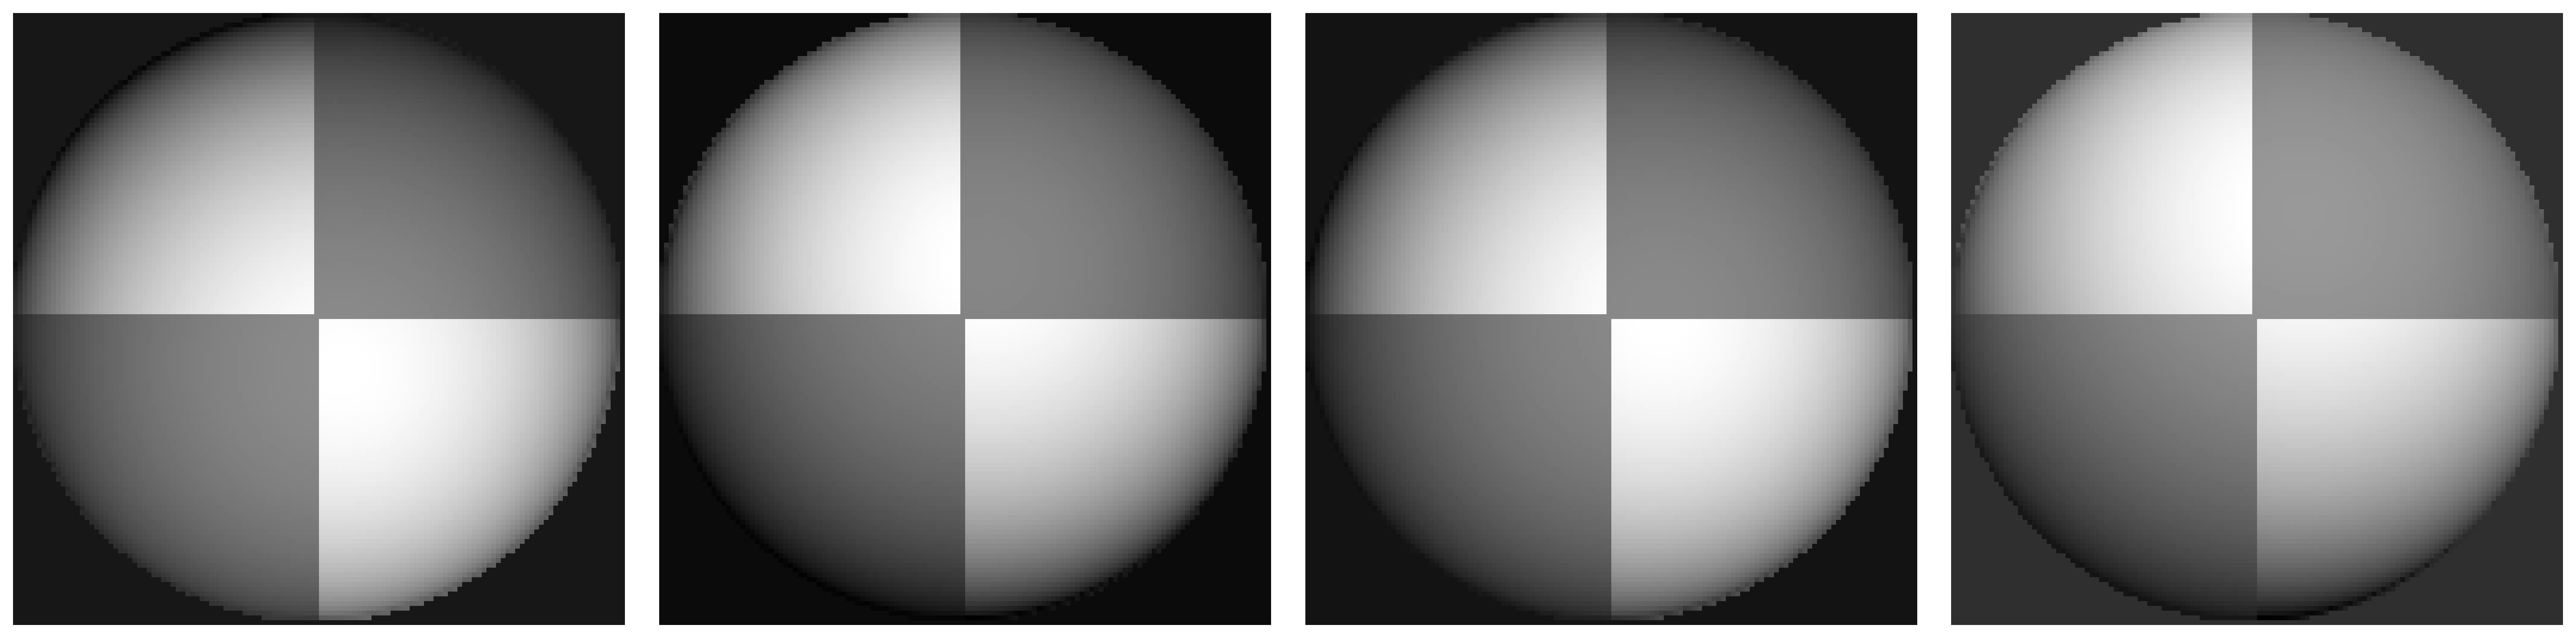
\includegraphics[width=\textwidth]{intensity_maps.png}
	\caption{Given 2D intensity maps of a 3D surface under varying illumination.}
	\label{fig:intensity}
\end{figure}

\begin{figure}[htb]
	\centering
	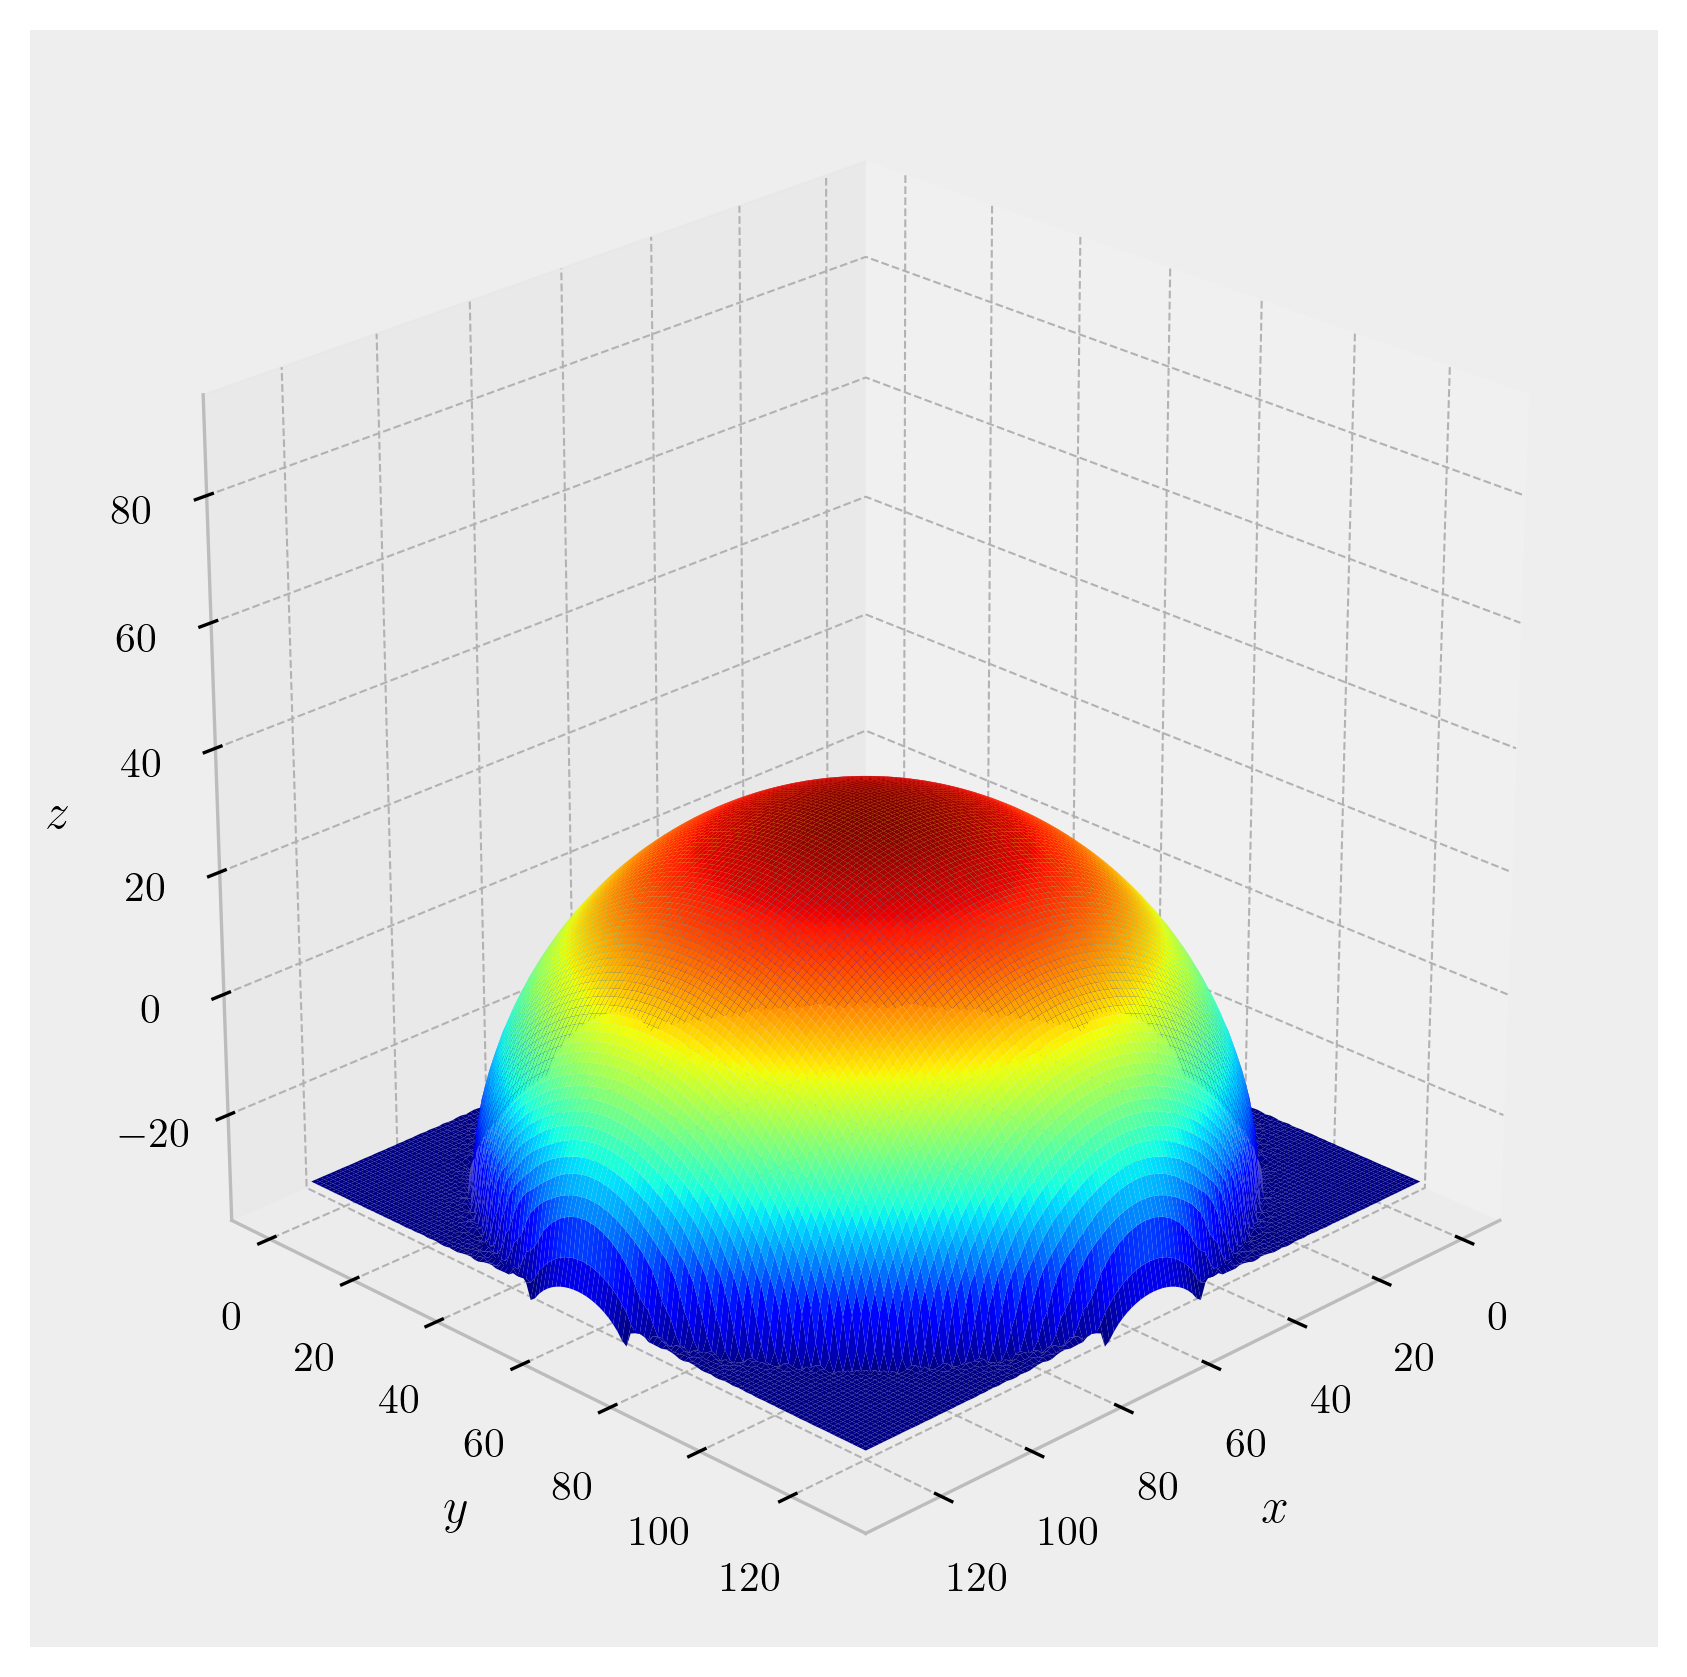
\includegraphics[width=\textwidth]{surface.png}
	\caption{Recovered surface.}
	\label{fig:surface}
\end{figure}


\bibliographystyle{spp-bst}
\bibliography{biblio}

\end{document}